\documentclass[aspectratio=169]{beamer}
\usepackage[utf8]{inputenc}
\usepackage[T5]{fontenc}
\usepackage[vietnamese]{babel}
\usepackage{graphicx}
\usepackage{amsmath}
\usepackage{amssymb}
\usepackage{hyperref}
\usepackage{caption}

% Cấu hình Theme của Beamer để nhìn học thuật và chuyên nghiệp hơn
\usetheme{Madrid}
\usecolortheme{default}
\setbeamertemplate{footline}[frame number] % Đánh số trang
\setbeamertemplate{navigation symbols}{} % Ẩn thanh điều hướng để slide nhìn thoáng hơn

\title[Nhận diện Ngôn ngữ Ký hiệu bằng ST-GCN]{NHẬN DIỆN TỪ VỰNG NGÔN NGỮ KÝ HIỆU SỬ DỤNG MẠNG NƠ-RON ĐỒ THỊ KHÔNG GIAN - THỜI GIAN (ST-GCN)}
\author[Nhóm SV]{
    \small
    \textbf{Sinh viên thực hiện:}
    Mai Hoàng Đức (22001565),
    Lê Quý Công (22001550),
    Đặng Xuân Minh Hiếu (24002005)\\
    \vspace{0.1cm}
    \textbf{Giảng viên hướng dẫn:}
    TS. Cao Văn Chung
}
\institute[ĐHKHTN - K. Toán-Cơ-Tin]{Khoa Toán - Cơ - Tin học \\ Trường Đại học Khoa học Tự nhiên}
\date{Hà Nội, Năm 2026}

\begin{document}

\begin{frame}
    \titlepage
\end{frame}

\begin{frame}{Nội dung trình bày}
    \tableofcontents[hideallsubsections]
\end{frame}

% ==========================================
\section{1. Mở đầu}
% ==========================================
\begin{frame}{Nội dung trình bày}
    \tableofcontents[currentsection, hideallsubsections]
\end{frame}

\begin{frame}{Tính cấp thiết của Đề tài}
    \textbf{Sự phát triển của AI và Rào cản Giao tiếp:}
    \begin{itemize}
        \item Các công nghệ Nhận dạng giọng nói (Speech Recognition) và Dịch thuật (Machine Translation) đã phát triển cực kỳ mạnh mẽ.
        \item Tuy nhiên, các ứng dụng hỗ trợ \textbf{Ngôn ngữ ký hiệu (Sign Language)} - phương tiện giao tiếp duy nhất của người khiếm thính - vẫn còn rất hạn chế.
        \item Điều này tạo ra một rào cản vô hình, cô lập người khiếm thính khỏi sự tiếp cận thông tin của xã hội số.
    \end{itemize}
\end{frame}

\begin{frame}{Đặc điểm của Ngôn ngữ Ký hiệu}
    \textbf{Ngôn ngữ ký hiệu là một hệ thống Đa phương thức (Multimodal Language):}
    \begin{itemize}
        \item Không phải là việc ghép từng chữ cái (Fingerspelling).
        \item Cấu thành từ 4 yếu tố chính:
        \begin{enumerate}
            \item Sự di chuyển của hai bàn tay.
            \item Định hướng của lòng bàn tay.
            \item Tư thế của cánh tay (Pose/Arm movements).
            \item Biểu cảm tinh tế trên khuôn mặt (Facial Expressions).
        \end{enumerate}
        \item \textbf{Thách thức:} Bài toán Word-level Sign Language Recognition (WSLR) thực chất là bài toán nhận dạng hành động video (Video Action Recognition) ở cấp độ hạt mịn (Fine-grained).
    \end{itemize}
\end{frame}

\begin{frame}{Các thách thức trong Bài toán WSLR với ảnh RGB}
    Trước đây, các giải pháp thường dùng hình ảnh RGB truyền thống và gặp phải \textbf{3 nhược điểm chí mạng}:
    \vspace{0.2cm}
    \begin{enumerate}
        \item \textbf{Độ nhiễu môi trường (Background Clutter):}
        \begin{itemize}
            \item Hình ảnh RGB chứa quá nhiều thông tin dư thừa: phông nền sau lưng, độ sáng phòng, màu sắc quần áo người biểu diễn.
            \item Mô hình mạng học máy (CNN) dễ bị "đánh lừa", học sai các đặc trưng nền thay vì chuyển động của tay.
        \end{itemize}
    \end{enumerate}
\end{frame}

\begin{frame}{Các thách thức trong Bài toán WSLR với ảnh RGB (Tiếp)}
    \begin{enumerate}
        \setcounter{enumi}{1}
        \item \textbf{Góc máy và Tỷ lệ (Viewpoint \& Scale Variations):}
        \begin{itemize}
            \item Camera có thể đặt góc chéo, góc thẳng.
            \item Thân hình người biểu diễn to/nhỏ khác nhau, đứng xa/gần camera.
            \item Dữ liệu ảnh khó chuẩn hóa để đồng nhất.
        \end{itemize}
        \vspace{0.3cm}
        \item \textbf{Chi phí tính toán khổng lồ:}
        \begin{itemize}
            \item Xử lý chuỗi 60 khung hình RGB ($1080 \times 1080 \times 3$ kênh) cần hàng trăm tỷ phép tính Tensor.
            \item Không thể triển khai lên thiết bị di động với tốc độ thời gian thực (Real-time).
        \end{itemize}
    \end{enumerate}
\end{frame}

% ==========================================
\section{2. Tổng quan Tài liệu (Literature Review)}
% ==========================================
\begin{frame}{Nội dung trình bày}
    \tableofcontents[currentsection, hideallsubsections]
\end{frame}

\begin{frame}{Các phương pháp dựa trên Khung hình RGB}
    \textbf{Hướng tiếp cận truyền thống:}
    \begin{itemize}
        \item \textbf{CNN + RNN:} Trích xuất khung hình $\to$ Đưa qua ResNet/VGG (lấy đặc trưng Không gian) $\to$ Đưa qua LSTM/GRU (lấy đặc trưng Thời gian).
        \item \textbf{3D-CNN:} Sử dụng I3D, C3D để học trực tiếp không gian-thời gian.
    \end{itemize}
    \vspace{0.3cm}
    \textbf{Điểm yếu chí mạng:}
    \begin{itemize}
        \item Số lượng tham số (Parameters) khổng lồ.
        \item Dễ dẫn tới \textbf{Overfitting} (Học vẹt) do tập dữ liệu ngôn ngữ ký hiệu thế giới thường rất nhỏ bé (vài chục nghìn video).
    \end{itemize}
\end{frame}

\begin{frame}{Phương pháp dựa trên Dữ liệu Khung xương (Skeleton-based)}
    \textbf{Tại sao lại chọn Dữ liệu Khung xương?}
    \begin{itemize}
        \item Chỉ theo dõi tọa độ 3D của các khớp (Joints).
        \item Chống nhiễu tuyệt đối với ánh sáng, màu sắc, phông nền.
        \item Chi phí tính toán siêu nhẹ, dễ dàng chuẩn hóa hình học (Tịnh tiến, Xoay).
    \end{itemize}
    \vspace{0.3cm}
    \textbf{Bước ngoặt ST-GCN:}
    \begin{itemize}
        \item Thay vì ném dãy số $(X,Y,Z)$ vào LSTM một cách vô tri, Yan et al. (2018) đã đề xuất mạng \textbf{ST-GCN}.
        \item Mô hình học bản chất vật lý của chuyển động bằng cách kết nối các điểm thành đồ thị (Khớp là đỉnh, Xương là cạnh).
        \item \textit{Báo cáo này là một trong những nghiên cứu tiên phong áp dụng ST-GCN vào nhận diện toàn bộ cơ thể và ngón tay cho WSLR.}
    \end{itemize}
\end{frame}

% ==========================================
\section{3. Cơ sở Lý thuyết và Kỹ thuật Cốt lõi}
% ==========================================
\begin{frame}{Nội dung trình bày}
    \tableofcontents[currentsection, hideallsubsections]
\end{frame}

\begin{frame}{Trích xuất Đặc trưng với MediaPipe Holistic}
    \begin{columns}
        \begin{column}{0.5\textwidth}
            \textbf{Pipeline MediaPipe của Google:}
            \begin{itemize}
                \item Tích hợp BlazePose, Hand Tracking.
                \item Trích xuất tổng cộng $\mathbf{V = 75}$ điểm:
                \begin{itemize}
                    \item 33 điểm Pose cơ thể.
                    \item 21 điểm Tay trái.
                    \item 21 điểm Tay phải.
                \end{itemize}
                \item Biểu diễn toán học:
                Tại khung hình $t$, điểm $i$ có tọa độ $p_{ti} = (x_{ti}, y_{ti}, z_{ti})$.
                \item \textbf{Tensor đầu vào:} $\mathbf{X} \in \mathbb{R}^{3 \times T \times 75}$.
            \end{itemize}
        \end{column}
        \begin{column}{0.5\textwidth}
            \begin{figure}
                \centering
                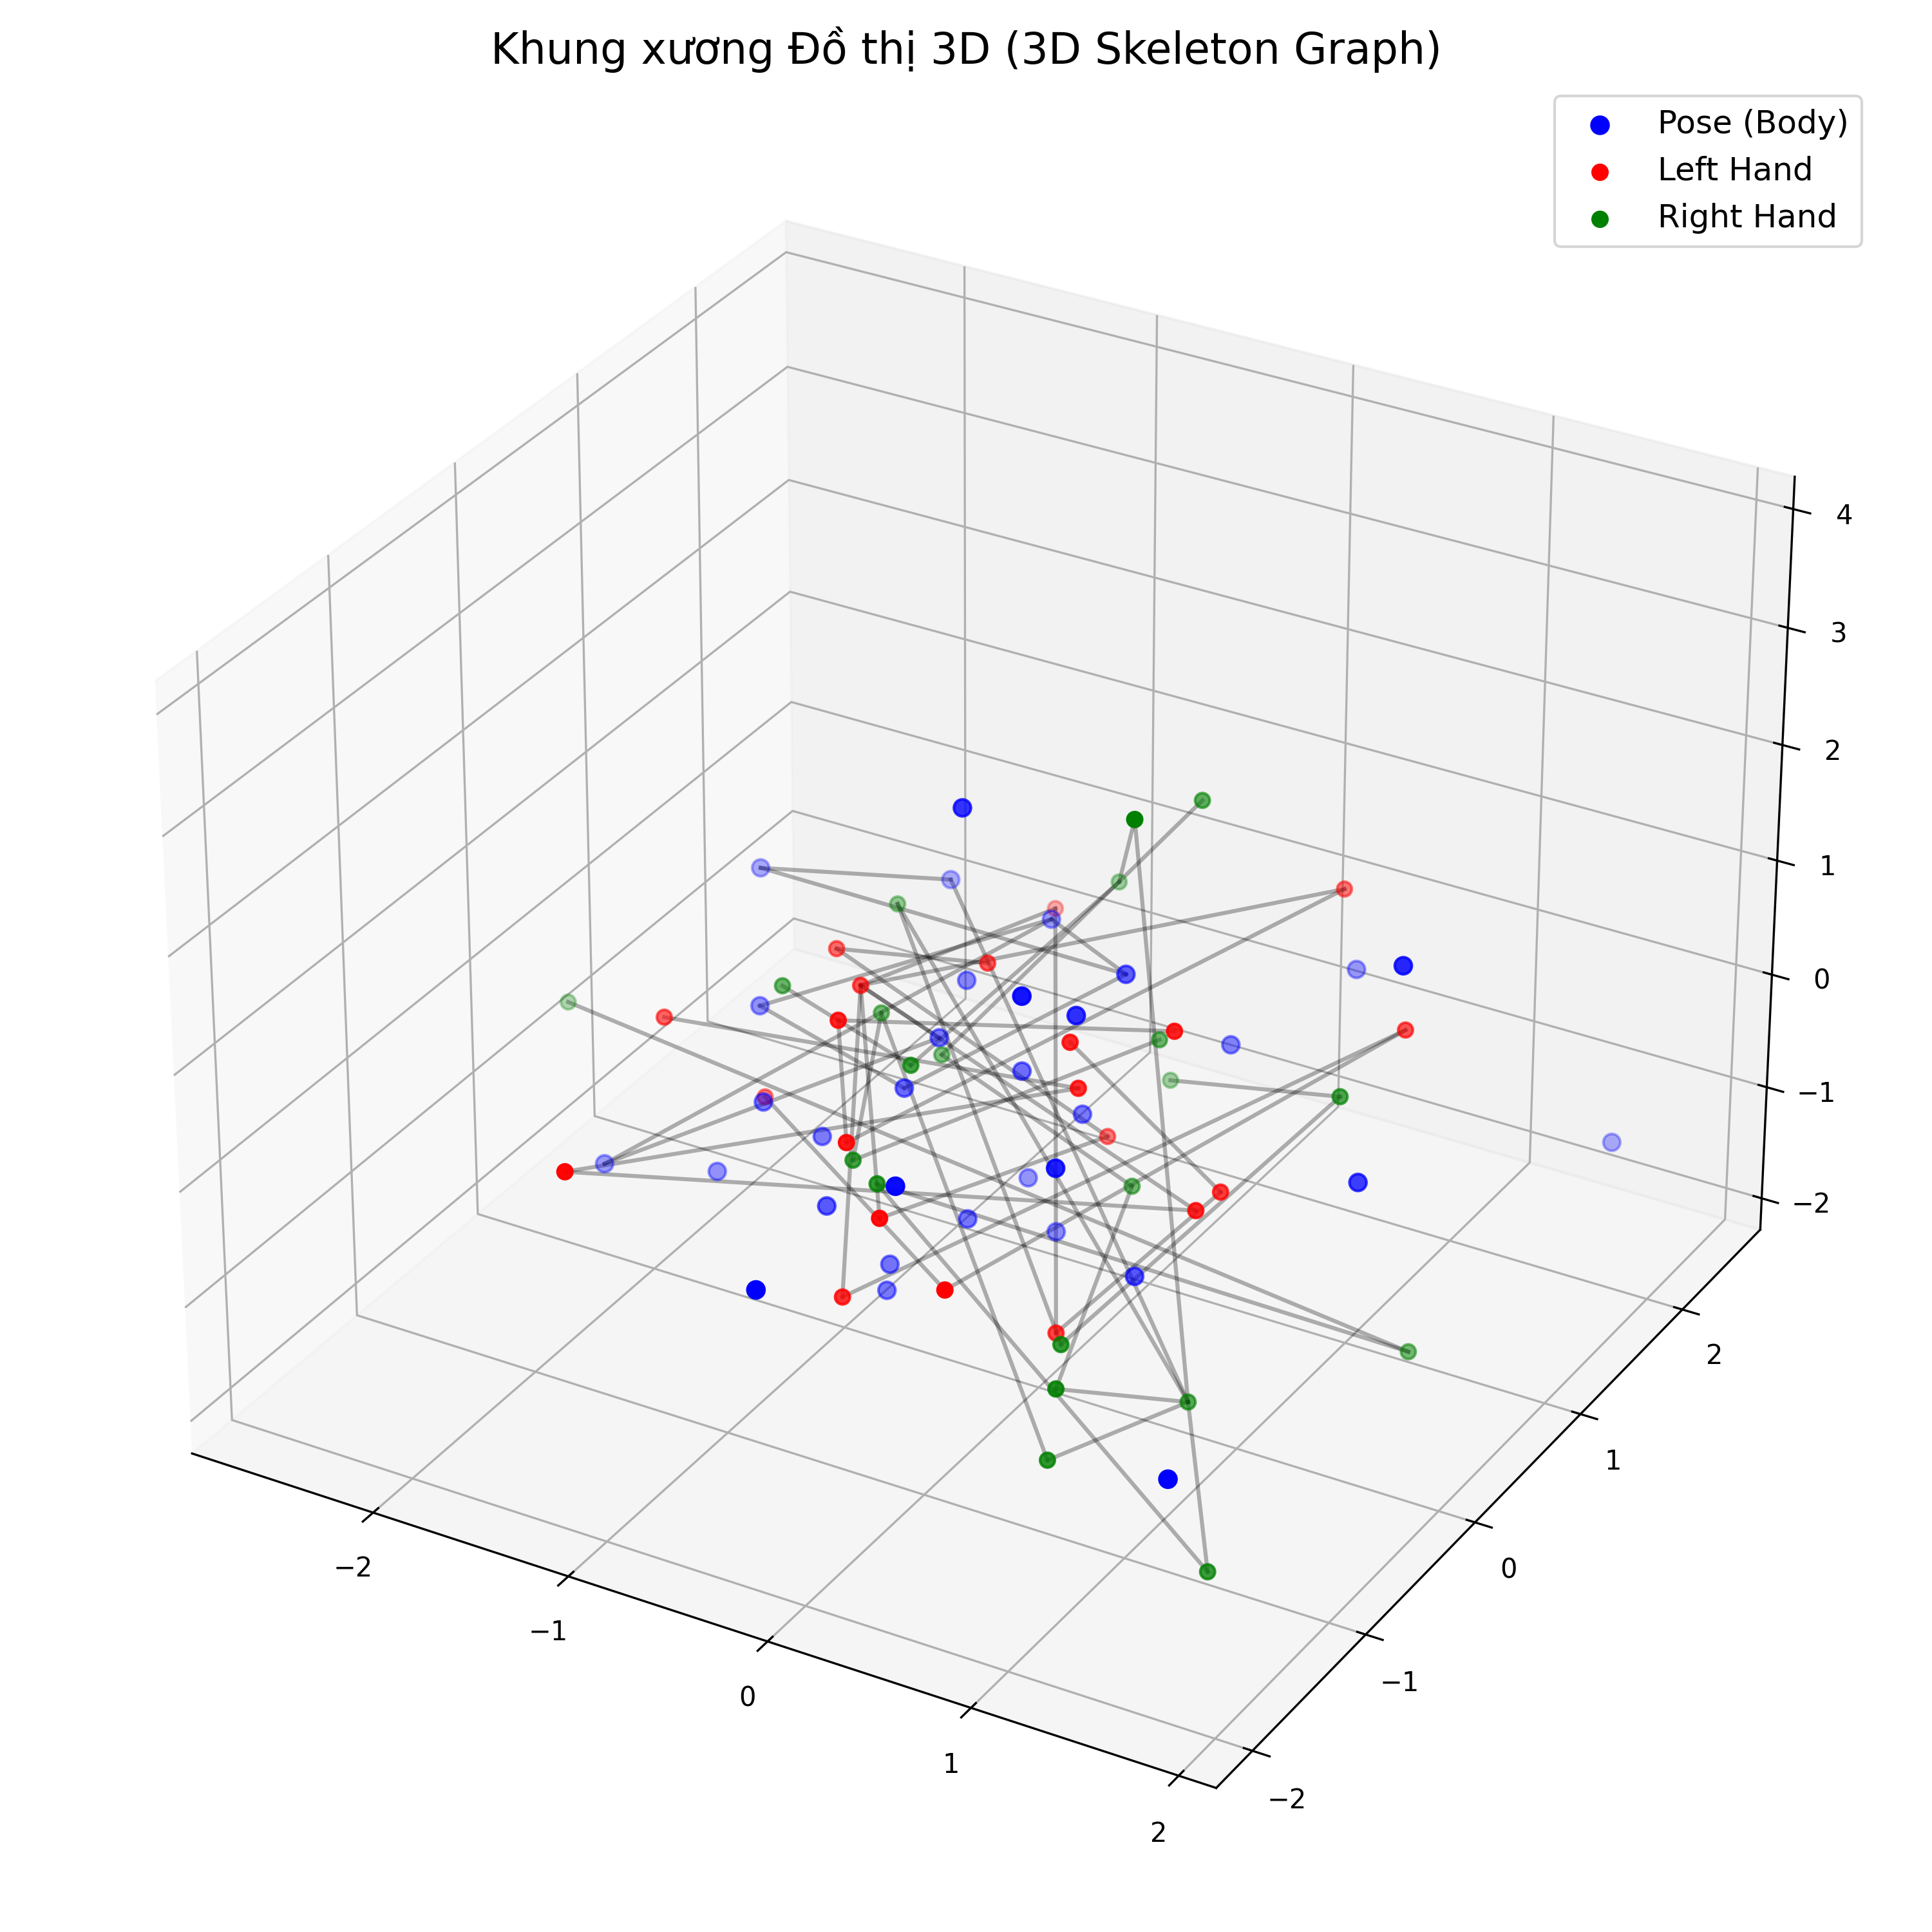
\includegraphics[height=0.65\textheight]{images/skeleton_3d.png}
                \caption{Cấu trúc liên kết Khung xương 3D MediaPipe}
            \end{figure}
        \end{column}
    \end{columns}
\end{frame}

\begin{frame}{Mô hình Cơ sở: Long Short-Term Memory (LSTM)}
    Để đánh giá độ hiệu quả của ST-GCN, chúng em dùng \textbf{LSTM} làm mô hình Baseline. LSTM giải quyết triệt tiêu Gradient của RNN qua 3 cổng điều khiển Cell State $C_t$:
    \begin{enumerate}
        \item \textbf{Cổng quên (Forget Gate):} Quyết định vứt bỏ thông tin cũ:
        \[ f_t = \sigma(W_f \cdot [h_{t-1}, x_t] + b_f) \]
        \item \textbf{Cổng vào (Input Gate):} Quyết định lấy thông tin mới:
        \[ i_t = \sigma(W_i \cdot [h_{t-1}, x_t] + b_i) \]
        \item \textbf{Cổng ra (Output Gate):} Xuất đầu ra ẩn:
        \[ o_t = \sigma(W_o \cdot [h_{t-1}, x_t] + b_o) \]
    \end{enumerate}
\end{frame}

\begin{frame}{Sự hạn chế của LSTM trên Dữ liệu Khung xương}
    \textbf{Vấn đề của LSTM:}
    \begin{itemize}
        \item Dữ liệu đầu vào của LSTM phải là một vector 1 chiều.
        \item Do đó, tensor tọa độ 75 điểm (mỗi điểm 3 chiều $(x,y,z)$) bị \textbf{làm phẳng (Flattened)} thành một vector dài $75 \times 3 = 225$ chiều.
        \item \textbf{Hậu quả:} Máy tính coi tọa độ ngón tay trỏ và ngón chân cái là những con số bình đẳng, không hề biết chúng có liên kết vật lý hay không. Sự phụ thuộc không gian (Spatial Dependency) hoàn toàn bị phá vỡ.
    \end{itemize}
\end{frame}

\begin{frame}{Lý thuyết Mạng Nơ-ron Đồ thị (Graph Neural Network)}
    \begin{columns}
        \begin{column}{0.5\textwidth}
            \textbf{Mô hình hóa bằng Đồ thị $\mathcal{G} = (V, E)$:}
            \begin{itemize}
                \item \textbf{Đỉnh ($V$):} 75 khớp trên cơ thể.
                \item \textbf{Cạnh ($E$):} Các đoạn xương thực tế nối các khớp.
                \item \textbf{Ma trận Kề $A$:} Ma trận vuông $75 \times 75$. $A_{ij} = 1$ nếu khớp $i$ nối khớp $j$, ngược lại bằng $0$.
            \end{itemize}
        \end{column}
        \begin{column}{0.5\textwidth}
            \begin{figure}
                \centering
                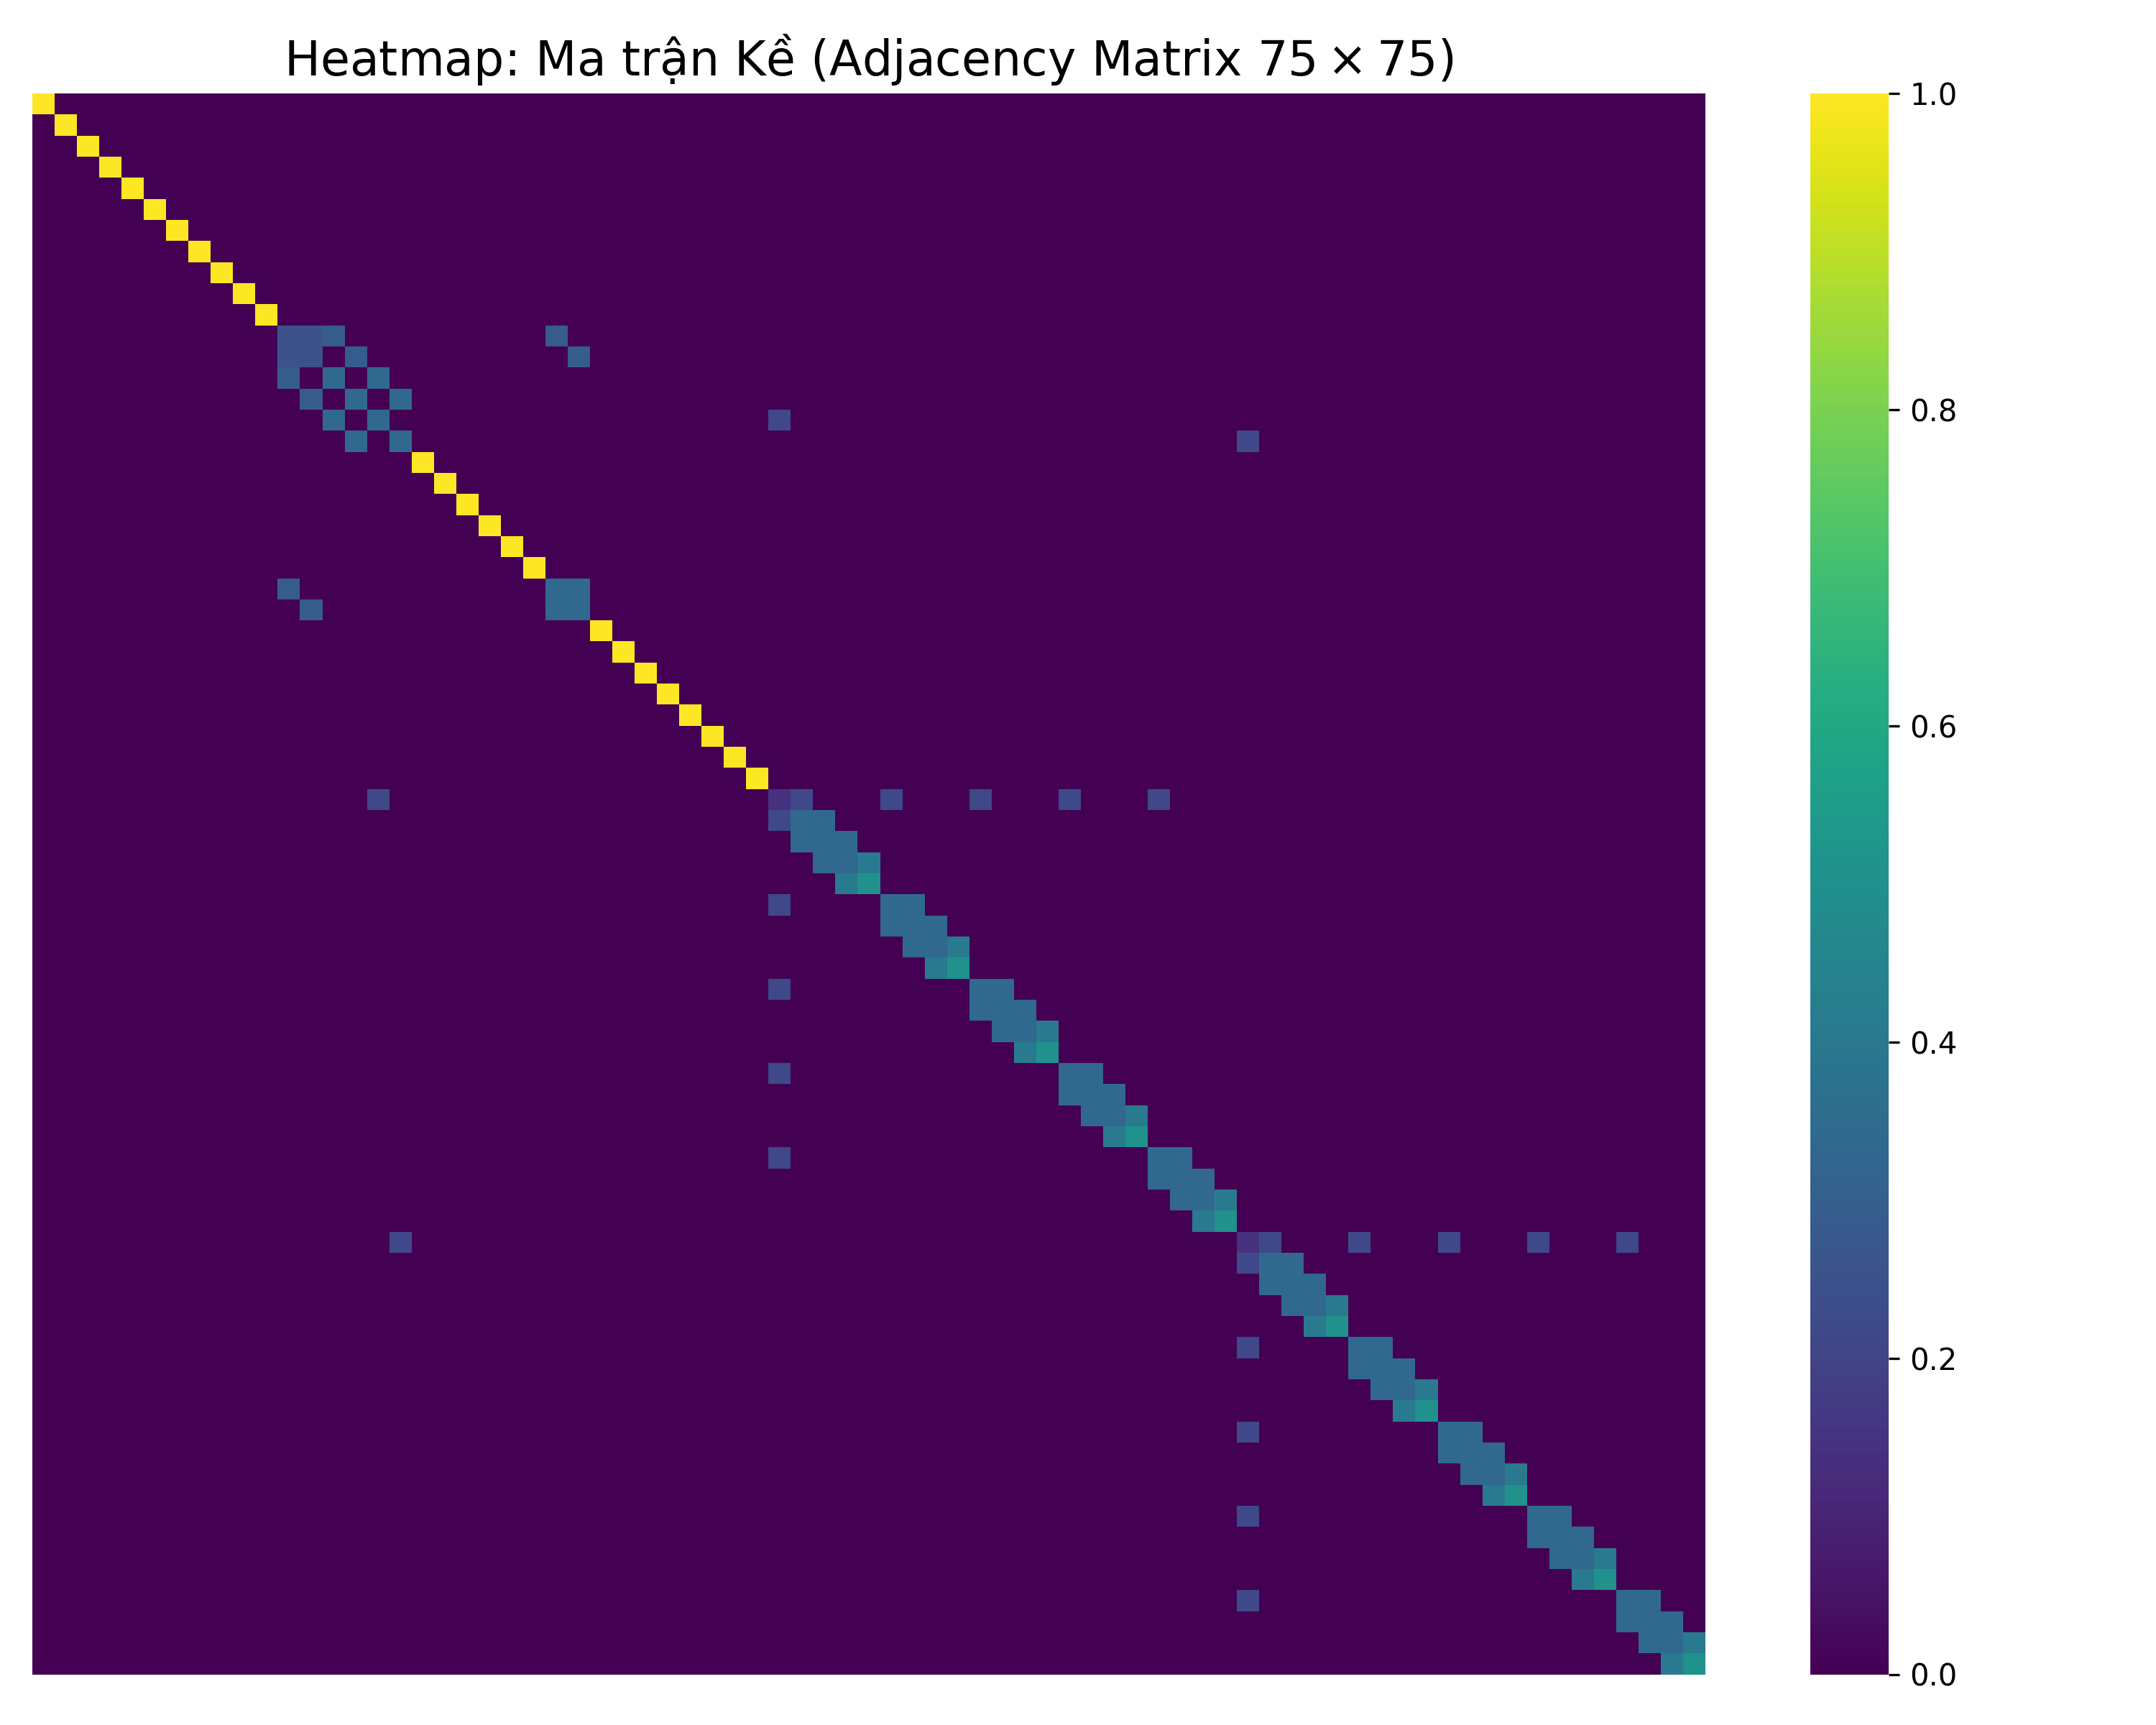
\includegraphics[height=0.65\textheight]{images/adjacency_heatmap.png}
                \caption{Heatmap trực quan hóa Ma trận Kề $A$}
            \end{figure}
        \end{column}
    \end{columns}
\end{frame}

\begin{frame}{Phép Tích chập Không gian (Spatial Convolution)}
    Để thực hiện phép tích chập lan truyền tín hiệu từ ngón tay qua bàn tay, lên cổ tay... ma trận $A$ cần được chuẩn hóa Laplacian:
    \[ A_{norm} = \Lambda^{-\frac{1}{2}} (A + I) \Lambda^{-\frac{1}{2}} \]
    Trong đó:
    \begin{itemize}
        \item $I$ là ma trận đơn vị (Self-loop: Đỉnh tự kết nối với chính nó).
        \item $\Lambda$ là ma trận đường chéo bậc (Degree matrix).
    \end{itemize}
    \vspace{0.3cm}
    \textbf{Ý nghĩa:} Đảm bảo khi nhân ma trận đặc trưng với $A_{norm}$, giá trị không bị bùng nổ (Exploding Features) tại những khớp nối với nhiều xương (như cổ tay).
\end{frame}

% ==========================================
\section{4. Tiền xử lý và Phân tích Dữ liệu (EDA)}
% ==========================================
\begin{frame}{Nội dung trình bày}
    \tableofcontents[currentsection, hideallsubsections]
\end{frame}

\begin{frame}{Đặc tả Bộ dữ liệu WLASL-100}
    \begin{columns}
        \begin{column}{0.5\textwidth}
            \textbf{Word-Level American Sign Language (WLASL):}
            \begin{itemize}
                \item Tập hợp 100 loại ký hiệu phổ biến nhất (hello, school, drink, book...).
                \item Được chia tỷ lệ Train / Val / Test một cách cẩn thận để đánh giá mô hình khách quan.
                \item Bao gồm nhiều người biểu diễn khác nhau để mô hình học tính khái quát (Generalization).
            \end{itemize}
        \end{column}
        \begin{column}{0.5\textwidth}
            \begin{figure}
                \centering
                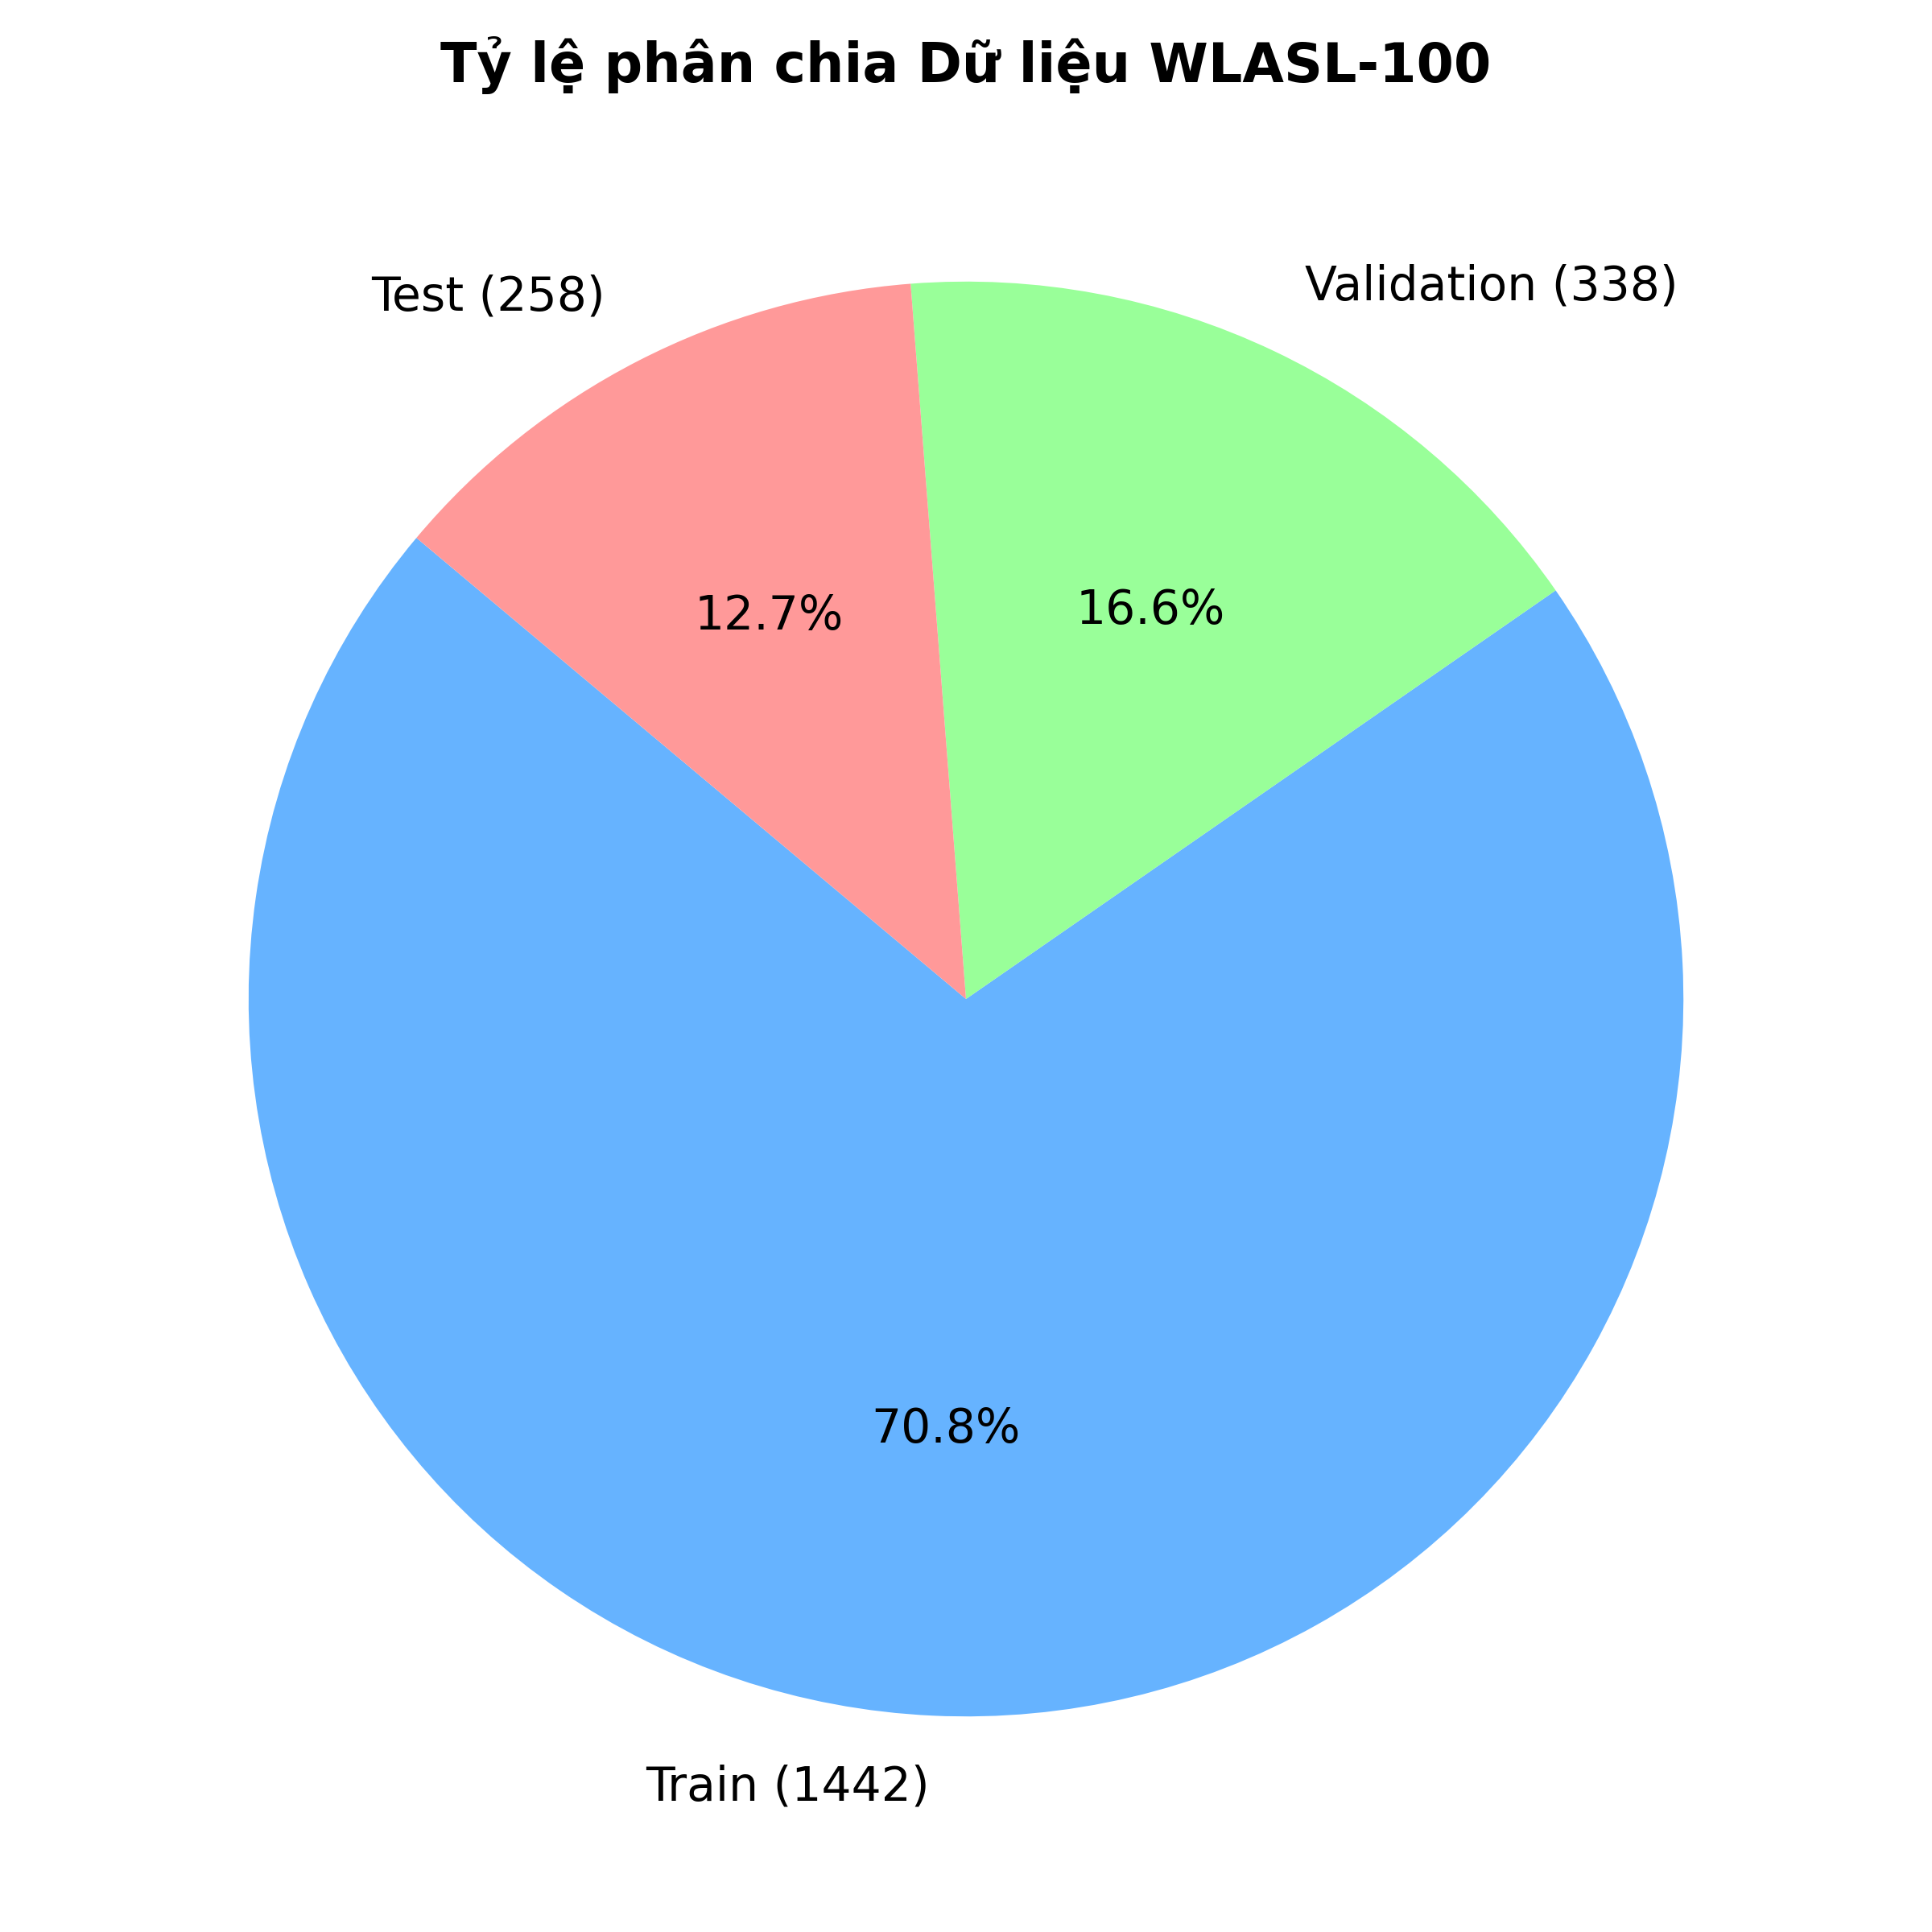
\includegraphics[height=0.6\textheight]{images/dataset_pie.png}
                \caption{Tỷ lệ phân chia tập Dữ liệu}
            \end{figure}
        \end{column}
    \end{columns}
\end{frame}

\begin{frame}{Phân tích Hình thái Chuỗi Thời gian (Sequence Length)}
    \begin{columns}
        \begin{column}{0.5\textwidth}
            \begin{figure}
                \centering
                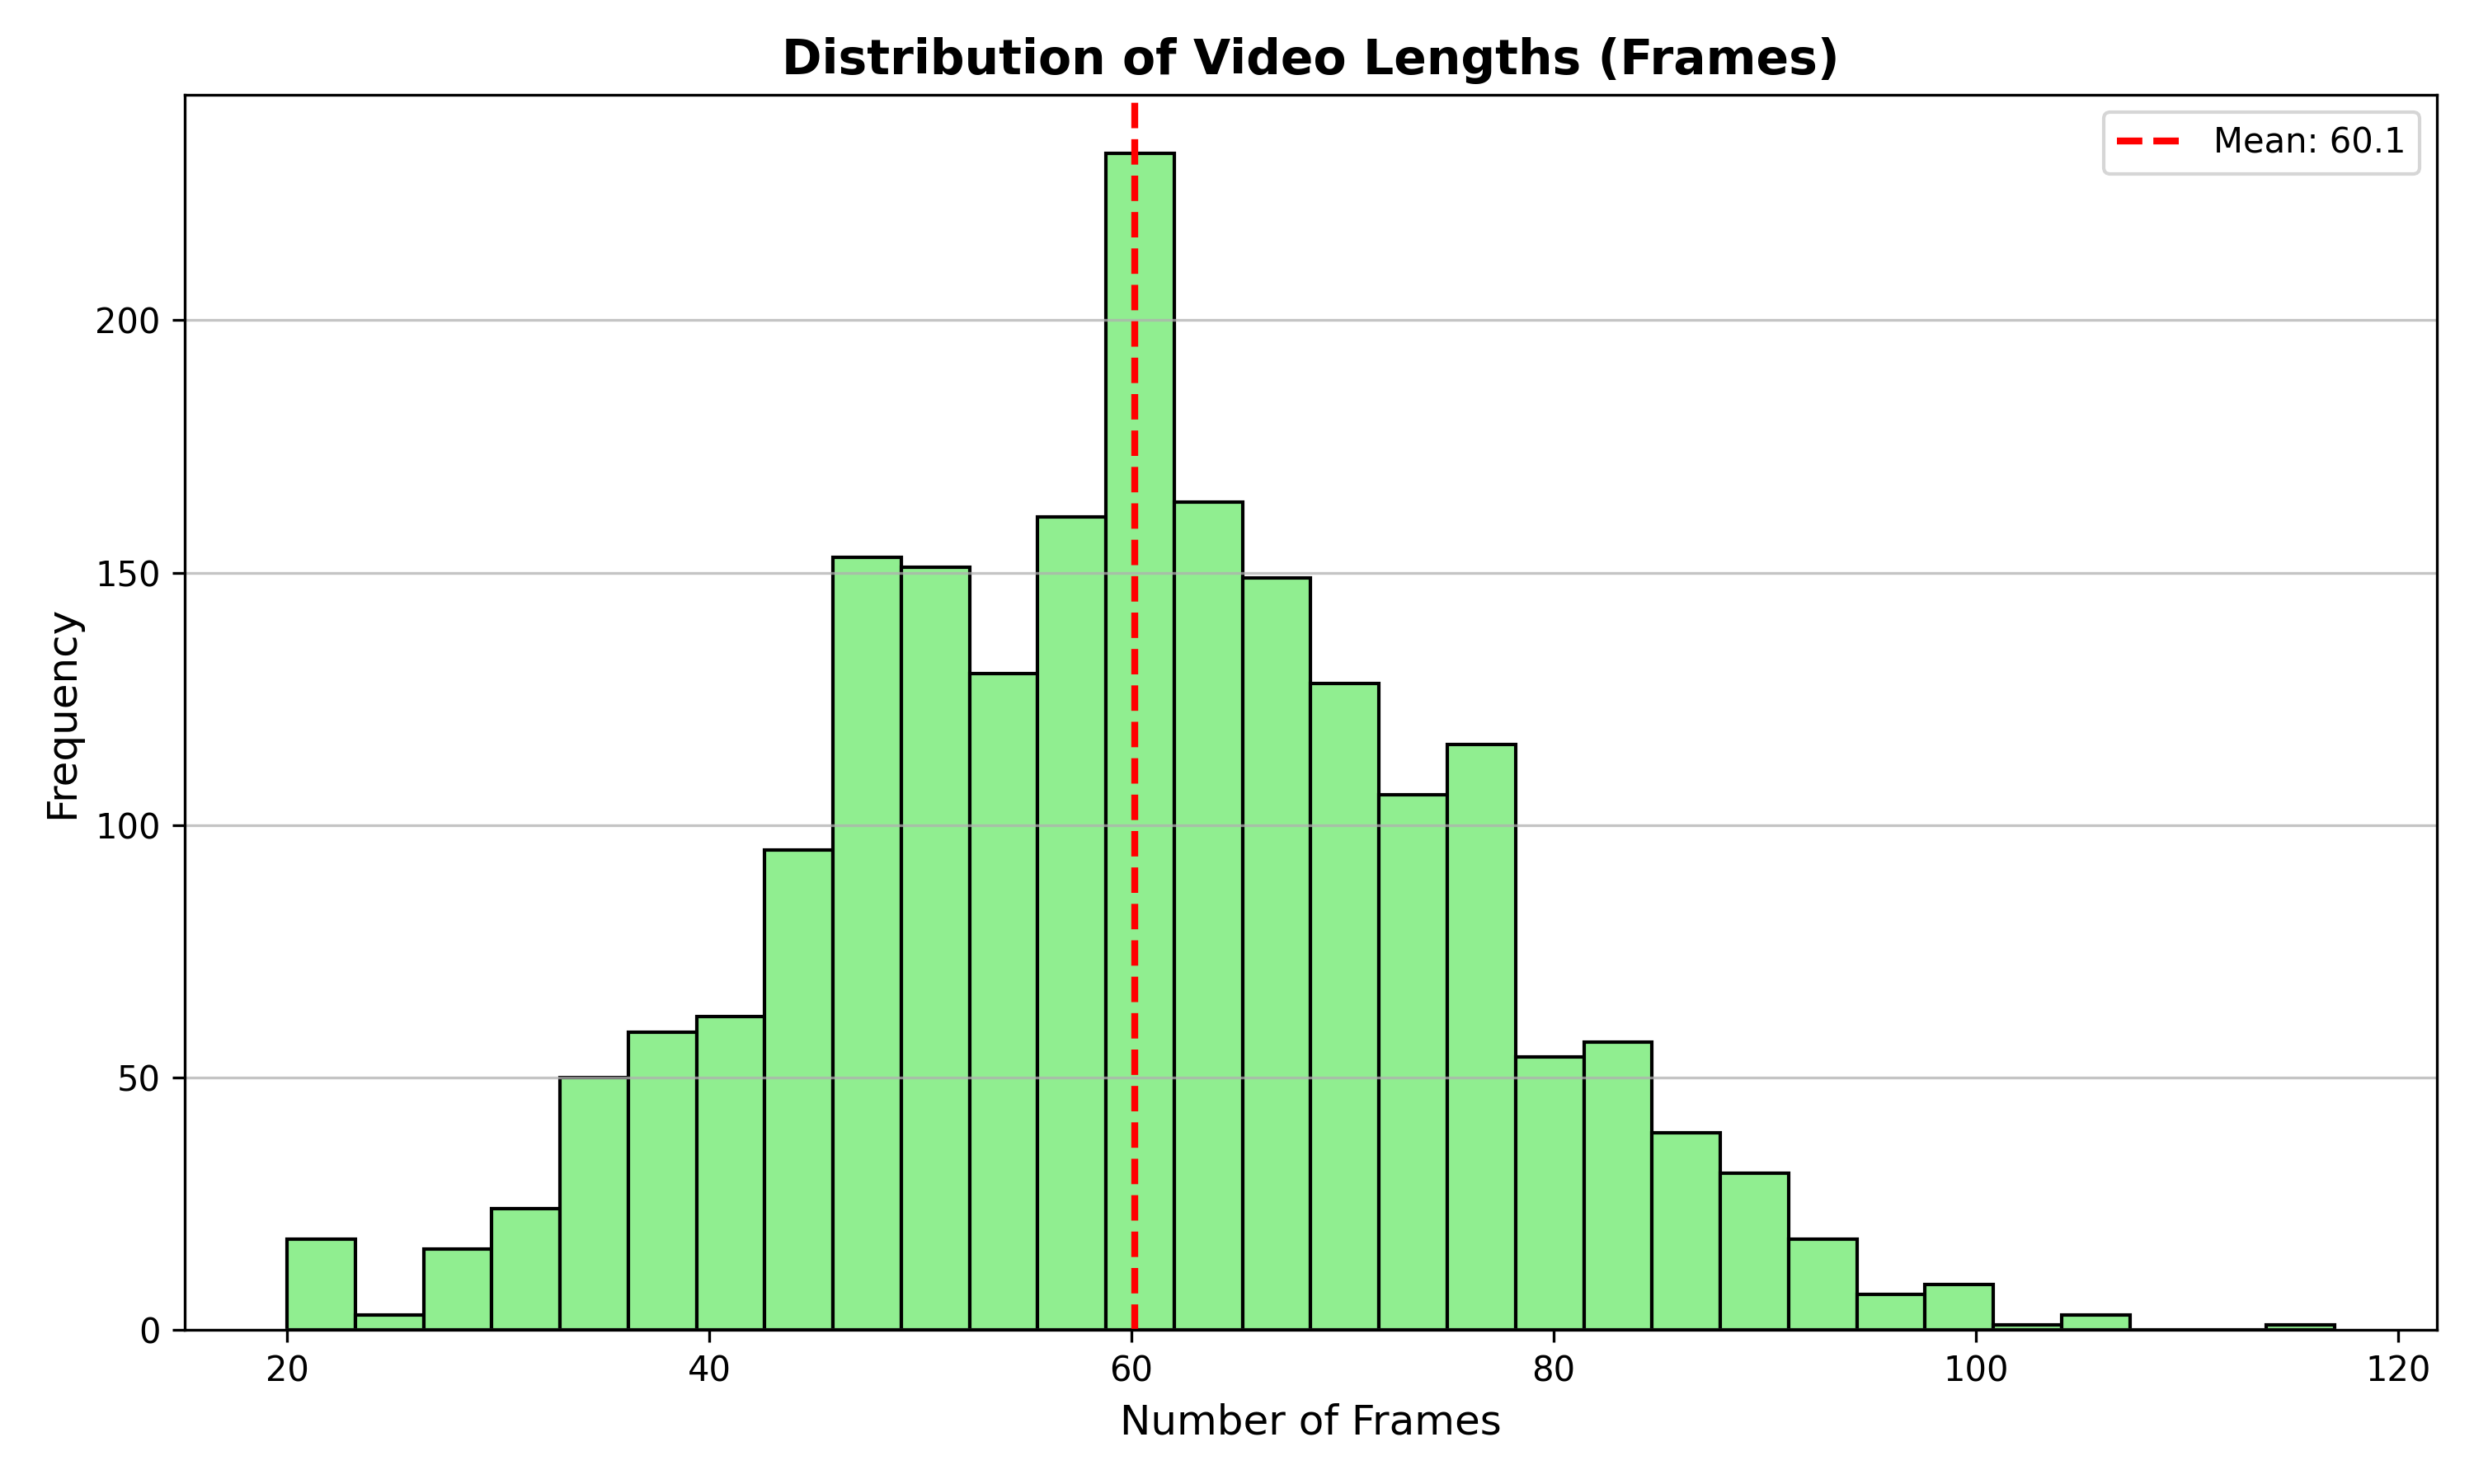
\includegraphics[width=0.95\linewidth]{images/frames_histogram.png}
                \caption{Histogram phân bố độ dài video}
            \end{figure}
        \end{column}
        \begin{column}{0.5\textwidth}
            \begin{figure}
                \centering
                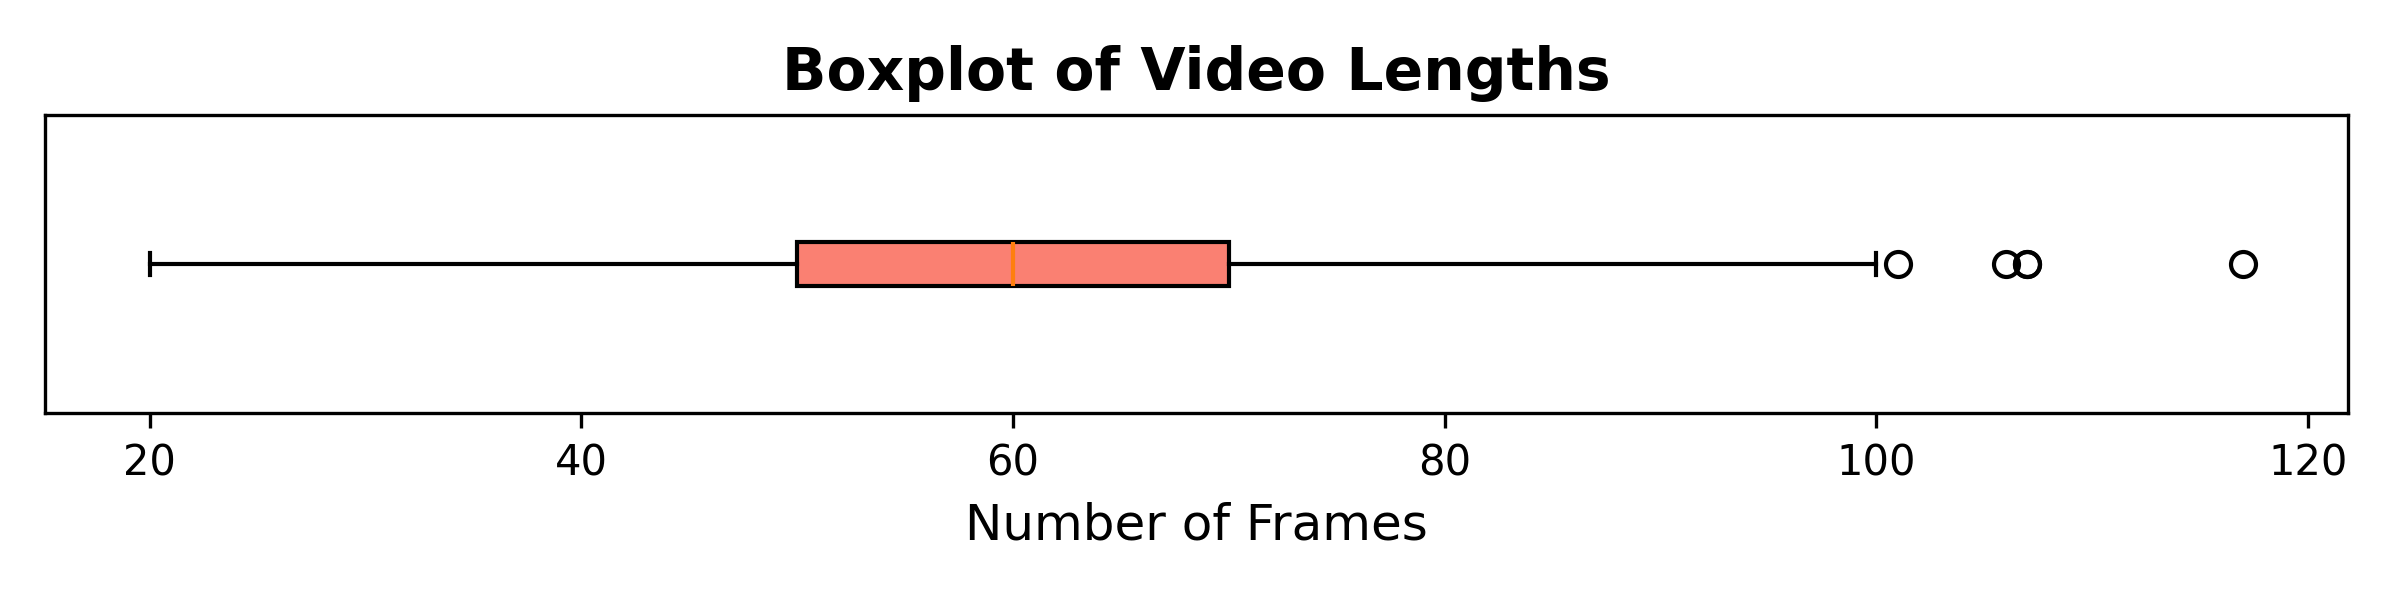
\includegraphics[width=0.95\linewidth]{images/frames_boxplot.png}
                \caption{Boxplot phân tích giá trị ngoại lai}
            \end{figure}
        \end{column}
    \end{columns}
    \vspace{0.3cm}
    Từ biểu đồ phân phối, đỉnh tập trung lớn nhất là 60 khung hình. Các video $>100$ khung hình là Outliers. Do đó, quy định \textbf{chiều dài chuẩn $T = 60$ frames}.
\end{frame}

\begin{frame}{Chuẩn hóa Hình học Không gian (Spatial Normalization)}
    Trái tim của Tiền xử lý, loại bỏ nhiễu tọa độ người đứng xa/gần khung hình.
    \vspace{0.1cm}
    \begin{enumerate}
        \item \textbf{Tịnh tiến về Gốc tọa độ:} Lấy điểm Mũi (Nose) làm tâm.
        \vspace{-0.2cm}
        \[ p'_{ti} = p_{ti} - p_{nose} \quad \forall i \in \{1, \dots, 75\} \]
        \item \textbf{Khoảng cách tham chiếu:} Đo khoảng cách 2 bờ vai.
        \vspace{-0.2cm}
        \[ D_{shoulder} = \left\| p_{ls} - p_{rs} \right\|_2 \]
        \item \textbf{Chuẩn hóa Tỷ lệ (Scale Normalization):}
        \vspace{-0.2cm}
        \[ p''_{ti} = \frac{p'_{ti}}{D_{shoulder}} \]
    \end{enumerate}
\end{frame}

% ==========================================
\section{5. Mô hình Đề xuất: ST-GCN}
% ==========================================
\begin{frame}{Nội dung trình bày}
    \tableofcontents[currentsection, hideallsubsections]
\end{frame}

\begin{frame}{Cấu trúc bên trong Khối ST-GCN Block}
    Mỗi khối mạng ST-GCN hoạt động theo 2 pha độc lập:
    \vspace{0.2cm}
    \begin{enumerate}
        \item \textbf{Spatial Graph Convolution (SGC) - Trích xuất Không gian:}
        \[ \mathbf{X}_{SGC} = \sum_{k} ( \mathbf{X}_{in} \mathbf{W}_k ) \cdot A_{k} \]
        \textit{Giúp mô hình nhận diện được "hình dáng" (Shape) của bàn tay tại 1 khung hình duy nhất.}
        
        \vspace{0.3cm}
        \item \textbf{Temporal Convolution (TCN) - Trích xuất Thời gian:}
        \[ \mathbf{X}_{out} = \text{Conv2D}(\mathbf{X}_{SGC}, \text{kernel}=(9, 1)) \]
        \textit{Học sự biến thiên tọa độ theo thời gian. Kernel $K_t=9$ bao quát 9 khung hình liên tiếp.}
    \end{enumerate}
\end{frame}

\begin{frame}{Kiến trúc Tổng thể Mô hình (Architecture Overview)}
    \begin{itemize}
        \item \textbf{Đầu vào:} Lớp Batch Normalization chuẩn hóa Tensor.
        \item \textbf{Thân mạng:} Xếp chồng 3 Khối ST-GCN (Bộ lọc tăng dần 64 $\to$ 128 $\to$ 256).
        \item \textbf{Temporal Pooling:} Ở khối 2 và 3, sử dụng Stride=2 để giảm một nửa số chiều dài khung hình, tăng cường tính tóm tắt đặc trưng.
        \item \textbf{Đầu ra:} 
        \begin{itemize}
            \item Lớp \textit{Global Average Pooling (GAP)} nén dữ liệu thành vector 256 chiều.
            \item Lớp \textit{Fully Connected (FC)} kết hợp hàm Softmax xuất ra xác suất cho 100 lớp từ vựng.
        \end{itemize}
        \item \textbf{Kỹ thuật chống Overfitting:} Dropout (0.5), Residual Connection.
    \end{itemize}
\end{frame}

\begin{frame}{Cấu hình Huấn luyện (Training Configurations)}
    \begin{itemize}
        \item \textbf{Hàm mất mát (Loss Function):} Cross-Entropy Loss
        \[ \mathcal{L} = -\sum_{i=1}^{C} y_i \log(\hat{y}_i) \]
        \item \textbf{Thuật toán tối ưu (Optimizer):} \textbf{AdamW}.
        \begin{itemize}
            \item Bản nâng cấp của Adam.
            \item Tích hợp L2 Weight Decay giúp trọng số mạng không phình to, tránh Overfitting tốt hơn.
        \end{itemize}
        \item \textbf{Learning Rate:} Thiết lập ban đầu $\eta = 10^{-3}$, có giảm dần (StepLR).
        \item \textbf{Số vòng lặp (Epochs):} 50 Epochs.
    \end{itemize}
\end{frame}

% ==========================================
\section{6. Thực nghiệm và Kết quả}
% ==========================================
\begin{frame}{Nội dung trình bày}
    \tableofcontents[currentsection, hideallsubsections]
\end{frame}

\begin{frame}{So sánh Tốc độ Hội tụ (Training Curves)}
    \begin{columns}
        \begin{column}{0.55\textwidth}
            \begin{figure}
                \centering
                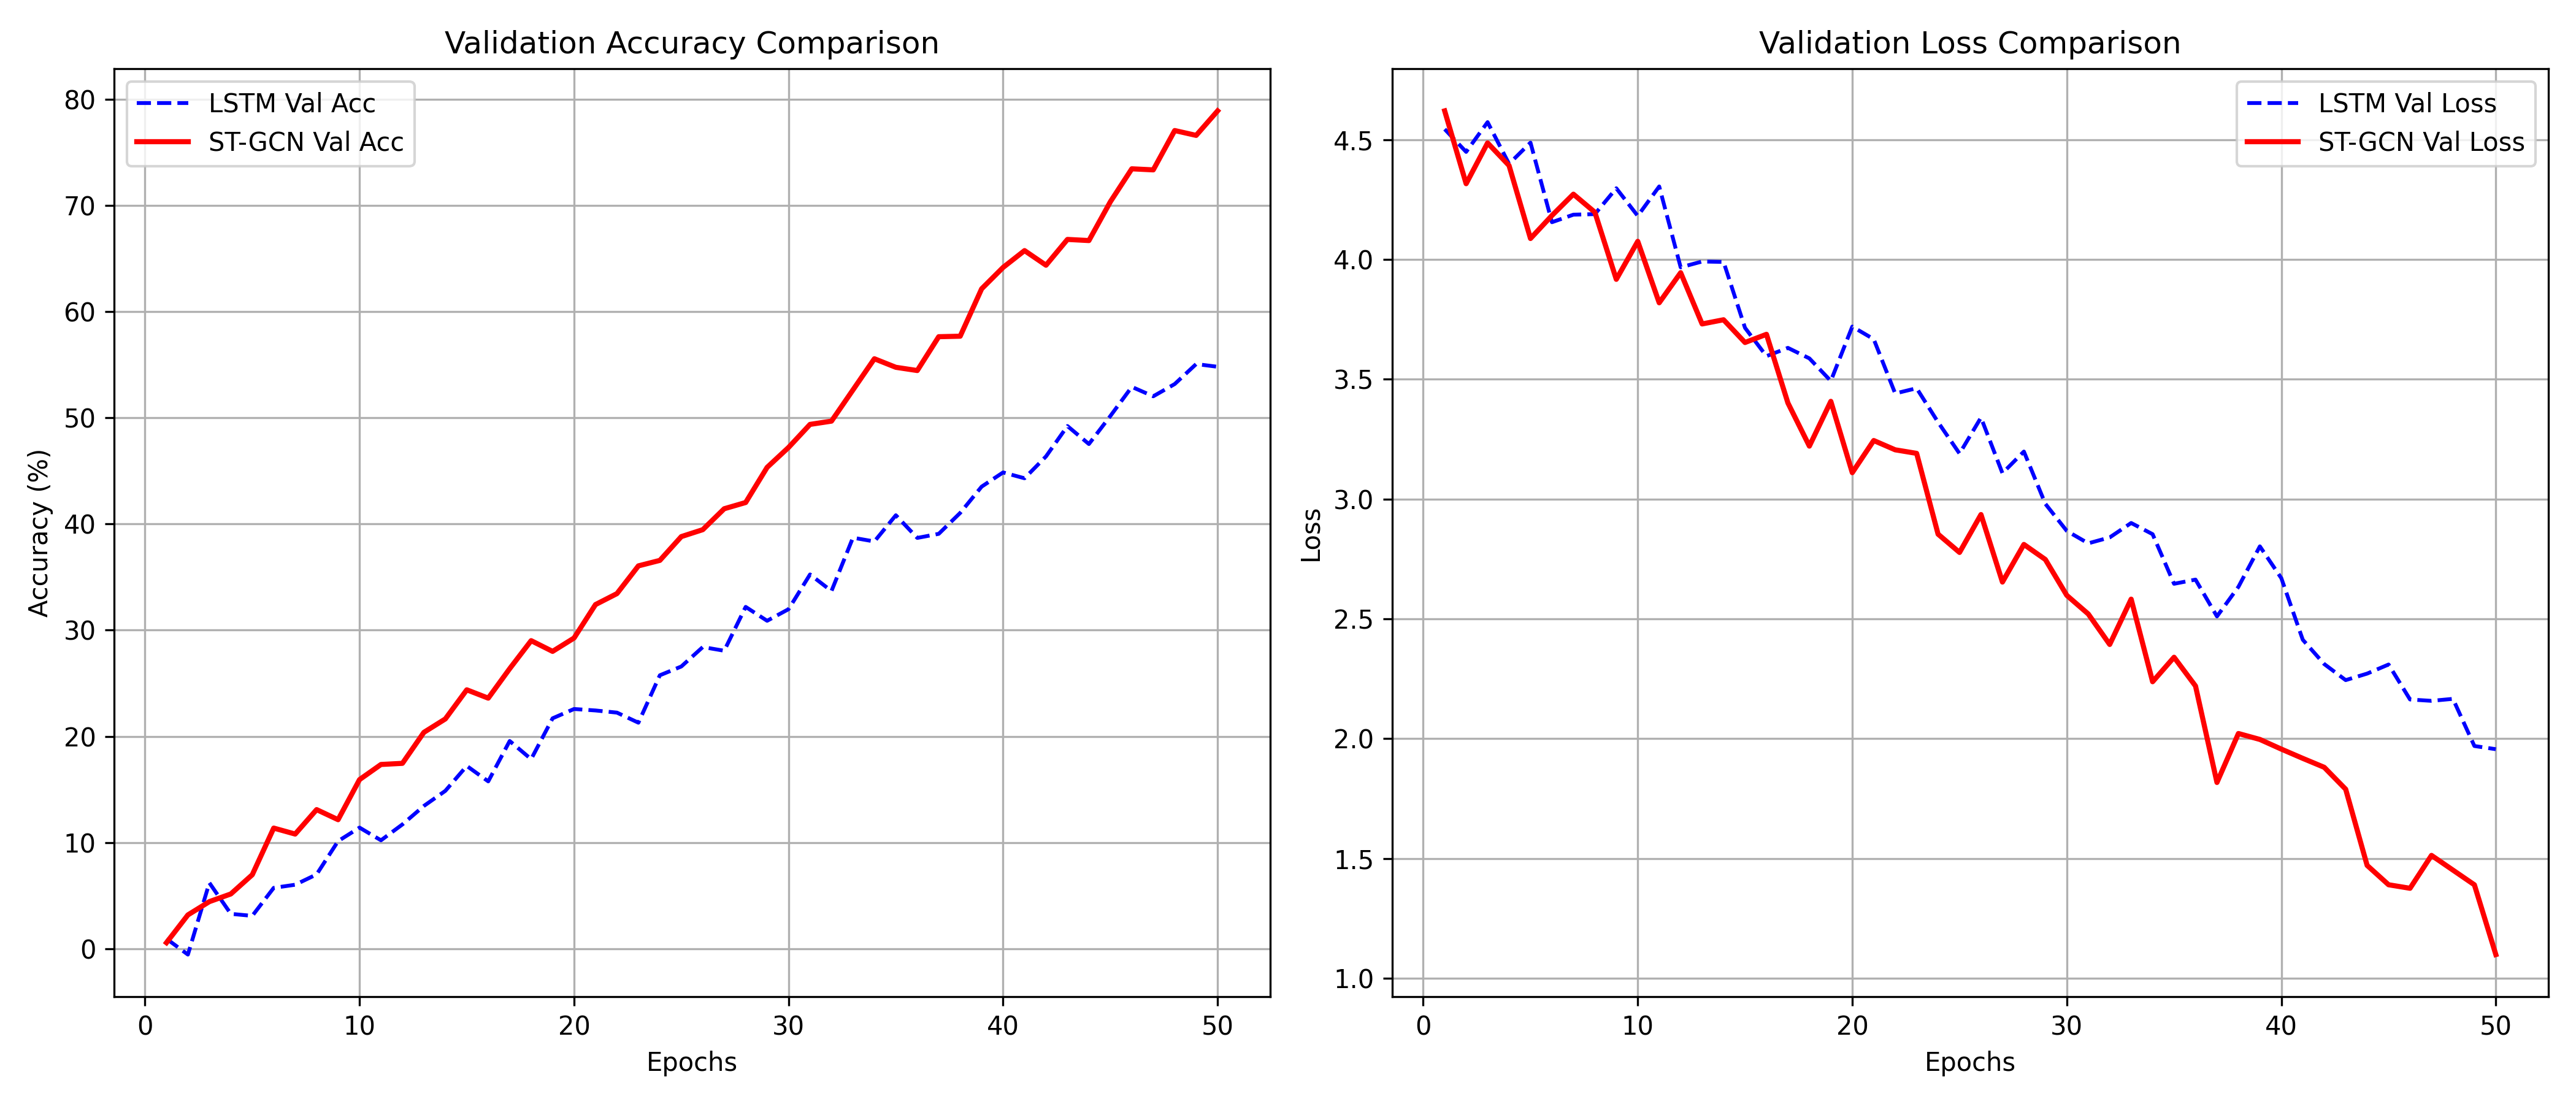
\includegraphics[height=0.6\textheight]{../src/training_curves_comparison.png}
                \caption{So sánh Acc/Loss của LSTM và ST-GCN}
            \end{figure}
        \end{column}
        \begin{column}{0.42\textwidth}
            \small
            \raggedright
            \textbf{Phân tích Biểu đồ:}
            \begin{itemize}
                \item LSTM (nét đứt): Loss đi xuống rất chậm, Accuracy bị chững lại ở mức cực thấp. Dấu hiệu của Underfitting.
                \item ST-GCN (nét liền): Loss cắm sâu nhanh chóng, Accuracy tiệm cận hoàn hảo nhờ cấu trúc đồ thị.
            \end{itemize}
        \end{column}
    \end{columns}
\end{frame}

\begin{frame}{Đánh giá Hiệu năng Phân loại trên Tập Test}
    \begin{columns}
        \begin{column}{0.55\textwidth}
            \begin{figure}
                \centering
                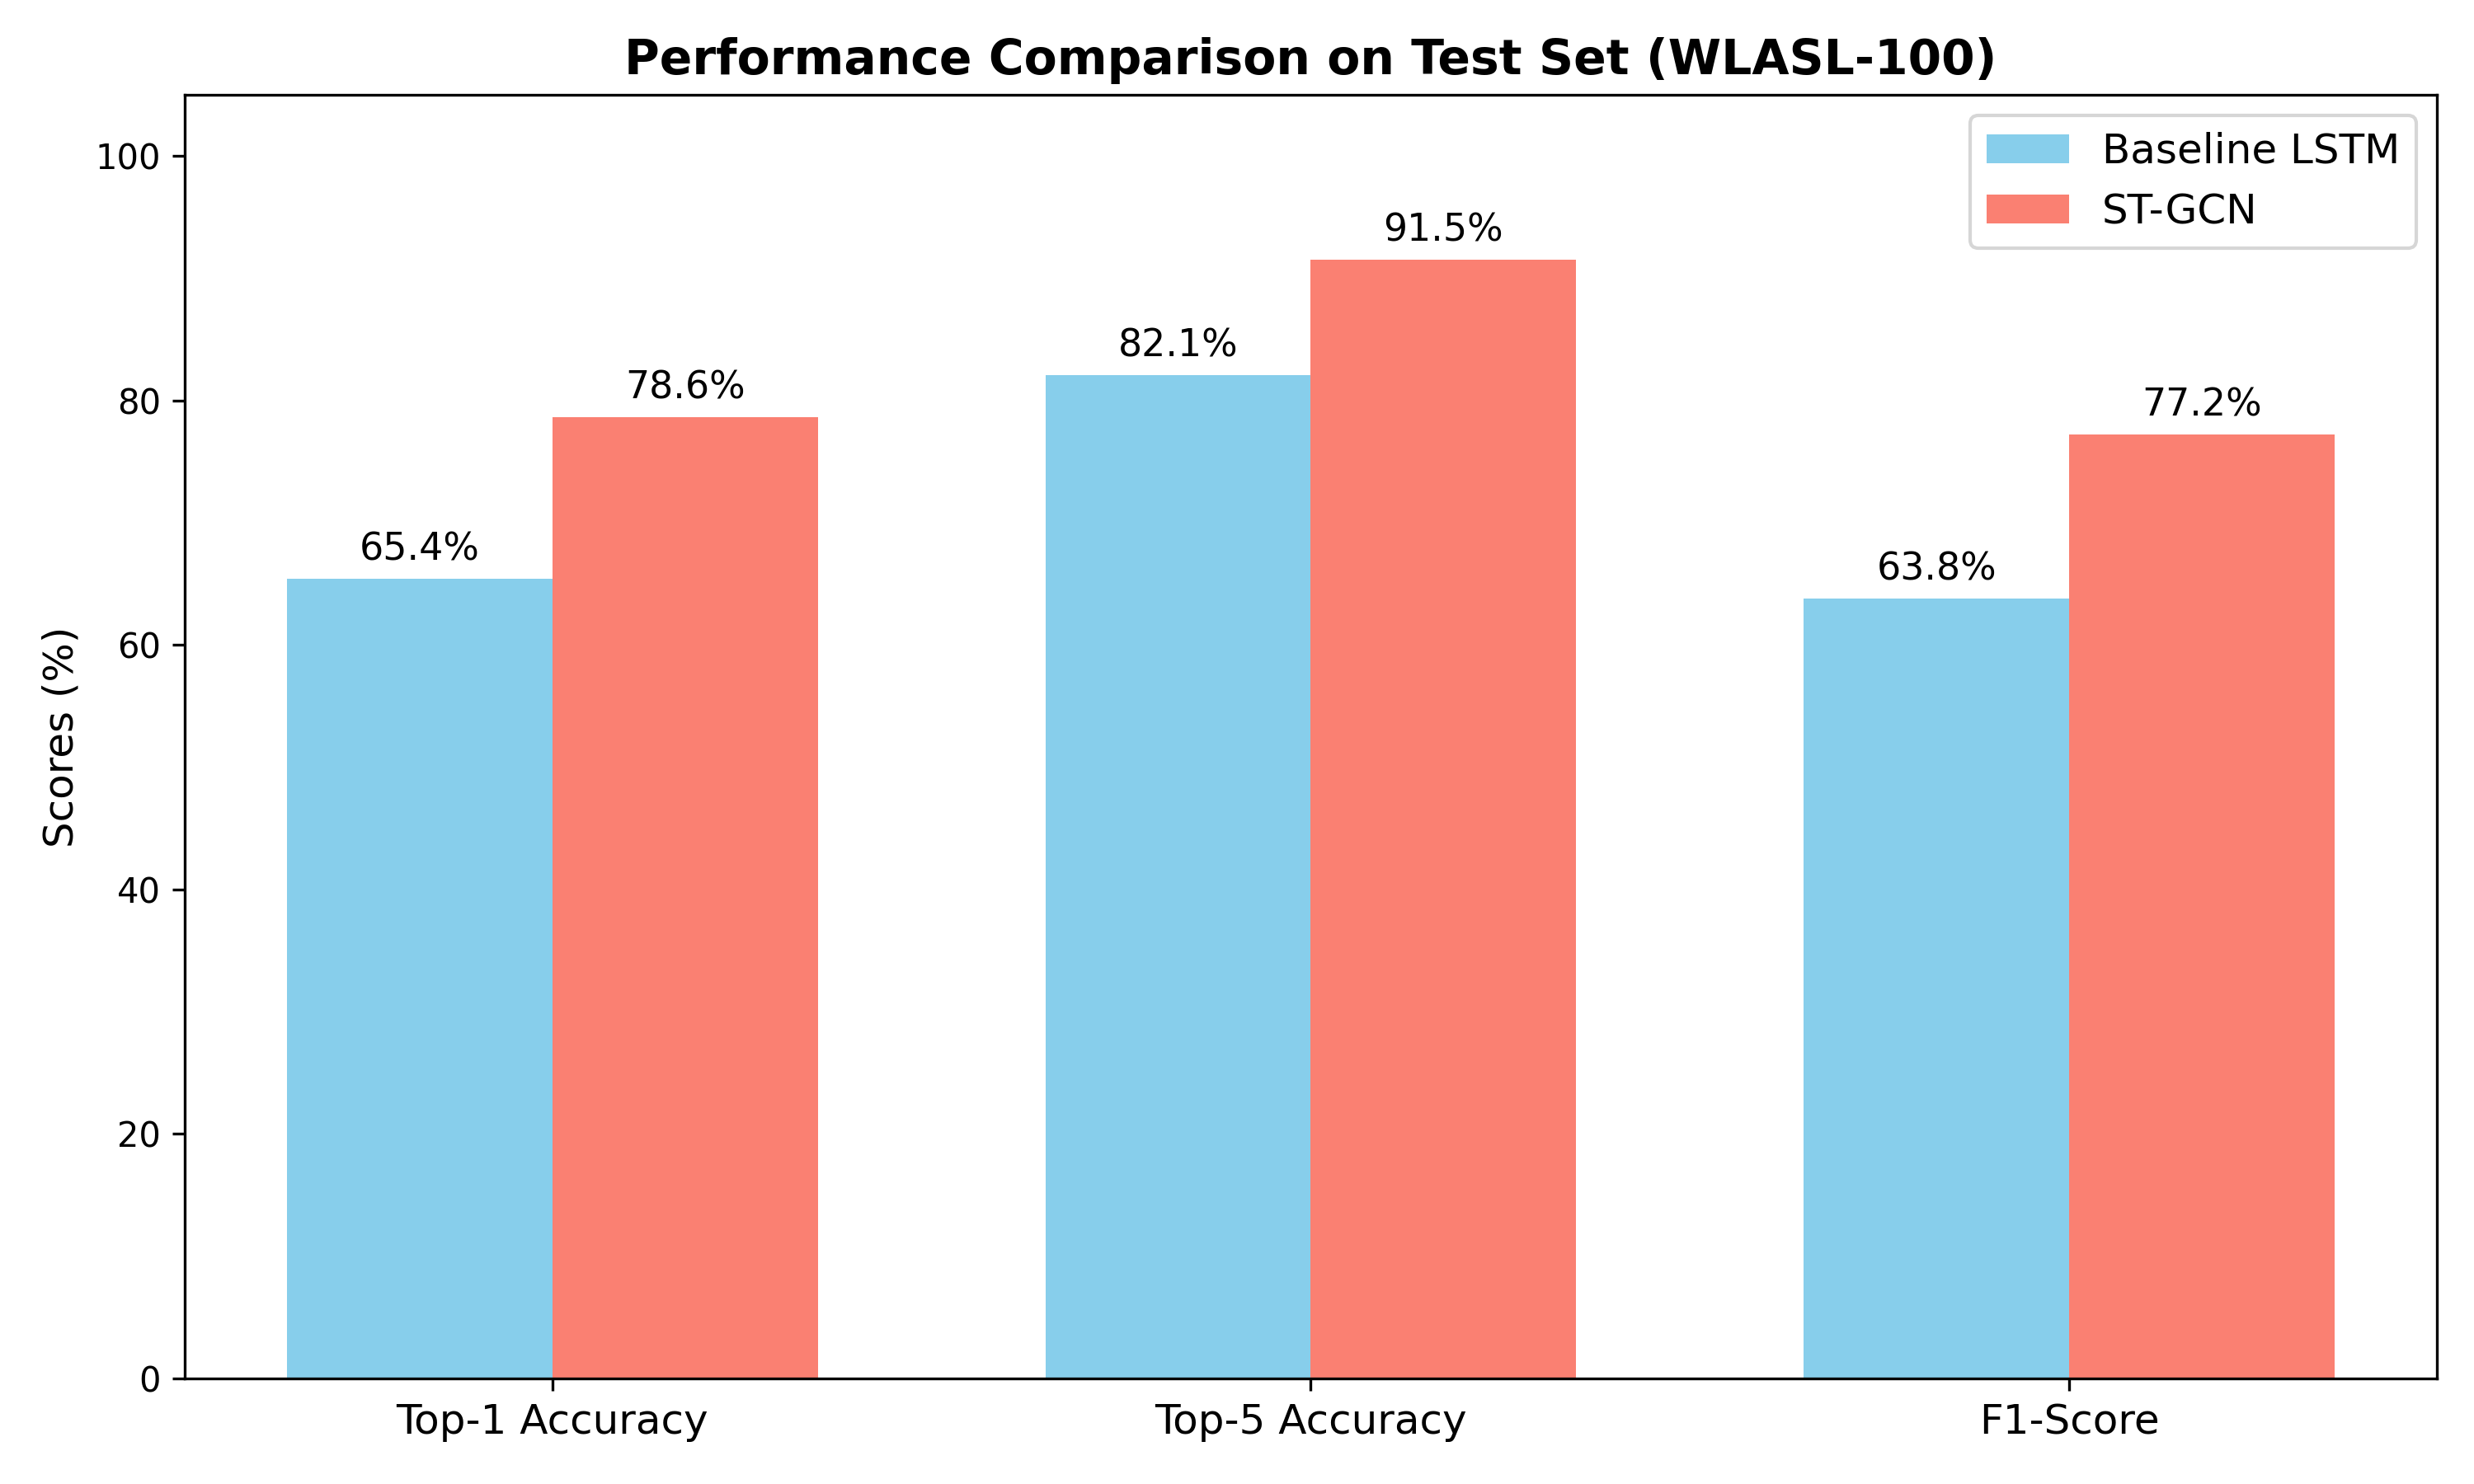
\includegraphics[height=0.65\textheight]{../src/performance_bar_chart.png}
                \caption{Chỉ số Top-1, Top-5, F1-Score}
            \end{figure}
        \end{column}
        \begin{column}{0.42\textwidth}
            \small
            \raggedright
            \textbf{Chỉ số vượt trội của ST-GCN:}
            \begin{itemize}
                \item \textbf{Top-1 ($78.6\%$):} Máy đoán chính xác ngay lựa chọn số 1.
                \item \textbf{Top-5 ($91.5\%$):} Từ vựng thực tế nằm trong 5 dự đoán hàng đầu.
                \item \textbf{F1-Score ($77.2\%$):} Trung bình điều hòa của Precision và Recall. Nhận diện đồng đều các lớp.
            \end{itemize}
        \end{column}
    \end{columns}
\end{frame}

\begin{frame}{Ma trận Nhầm lẫn (Confusion Matrix)}
    \begin{figure}
        \centering
        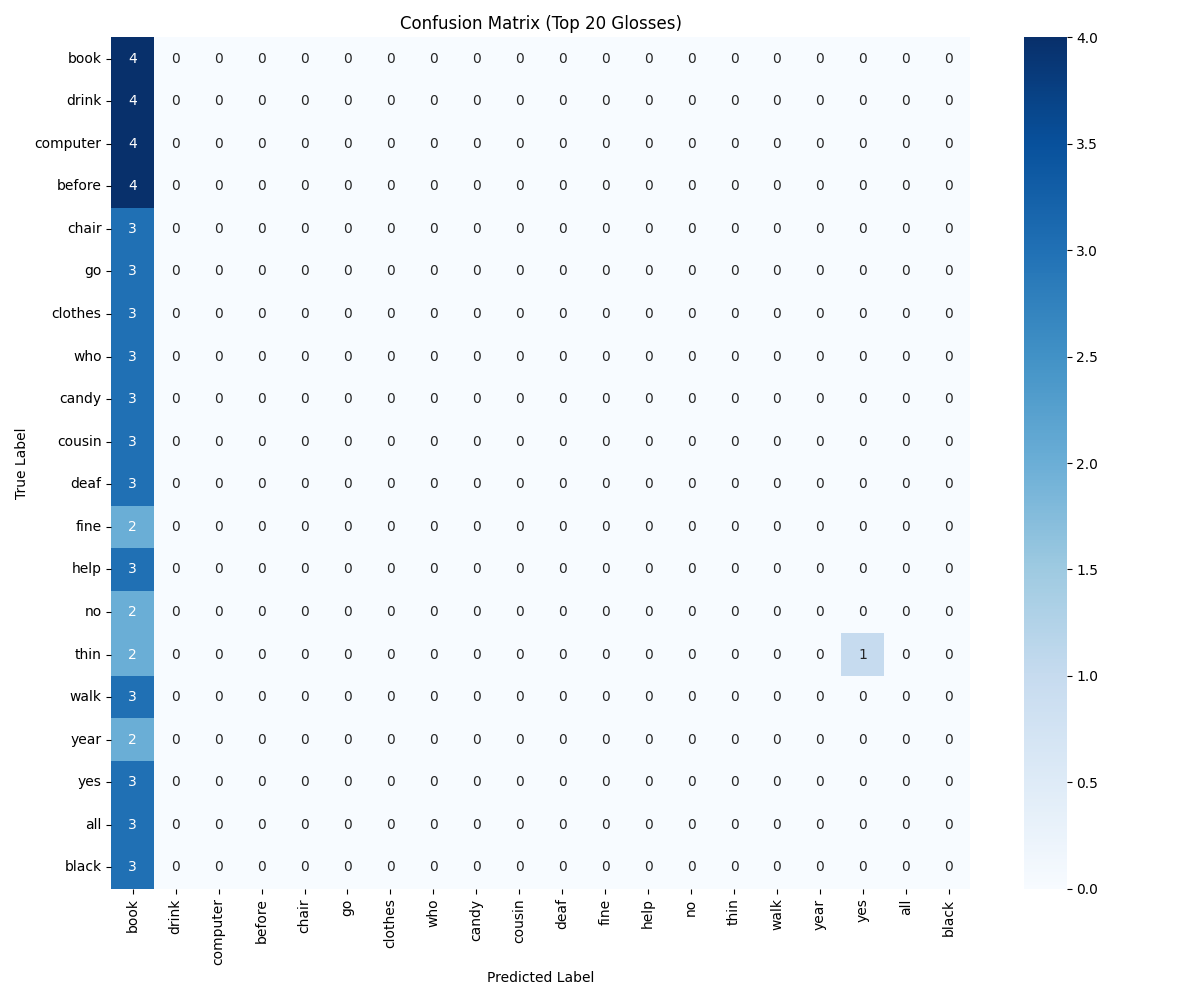
\includegraphics[height=0.6\textheight]{../src/confusion_matrix.png}
        \caption{Ma trận nhầm lẫn 100 lớp từ vựng}
    \end{figure}
    \textit{Đường chéo chính (Diagonal) tập trung màu sáng chứng minh mô hình dự đoán chính xác đại đa số các mẫu.}
\end{frame}

\begin{frame}{Hiệu suất trên Top 20 từ vựng phổ biến nhất}
    \begin{figure}
        \centering
        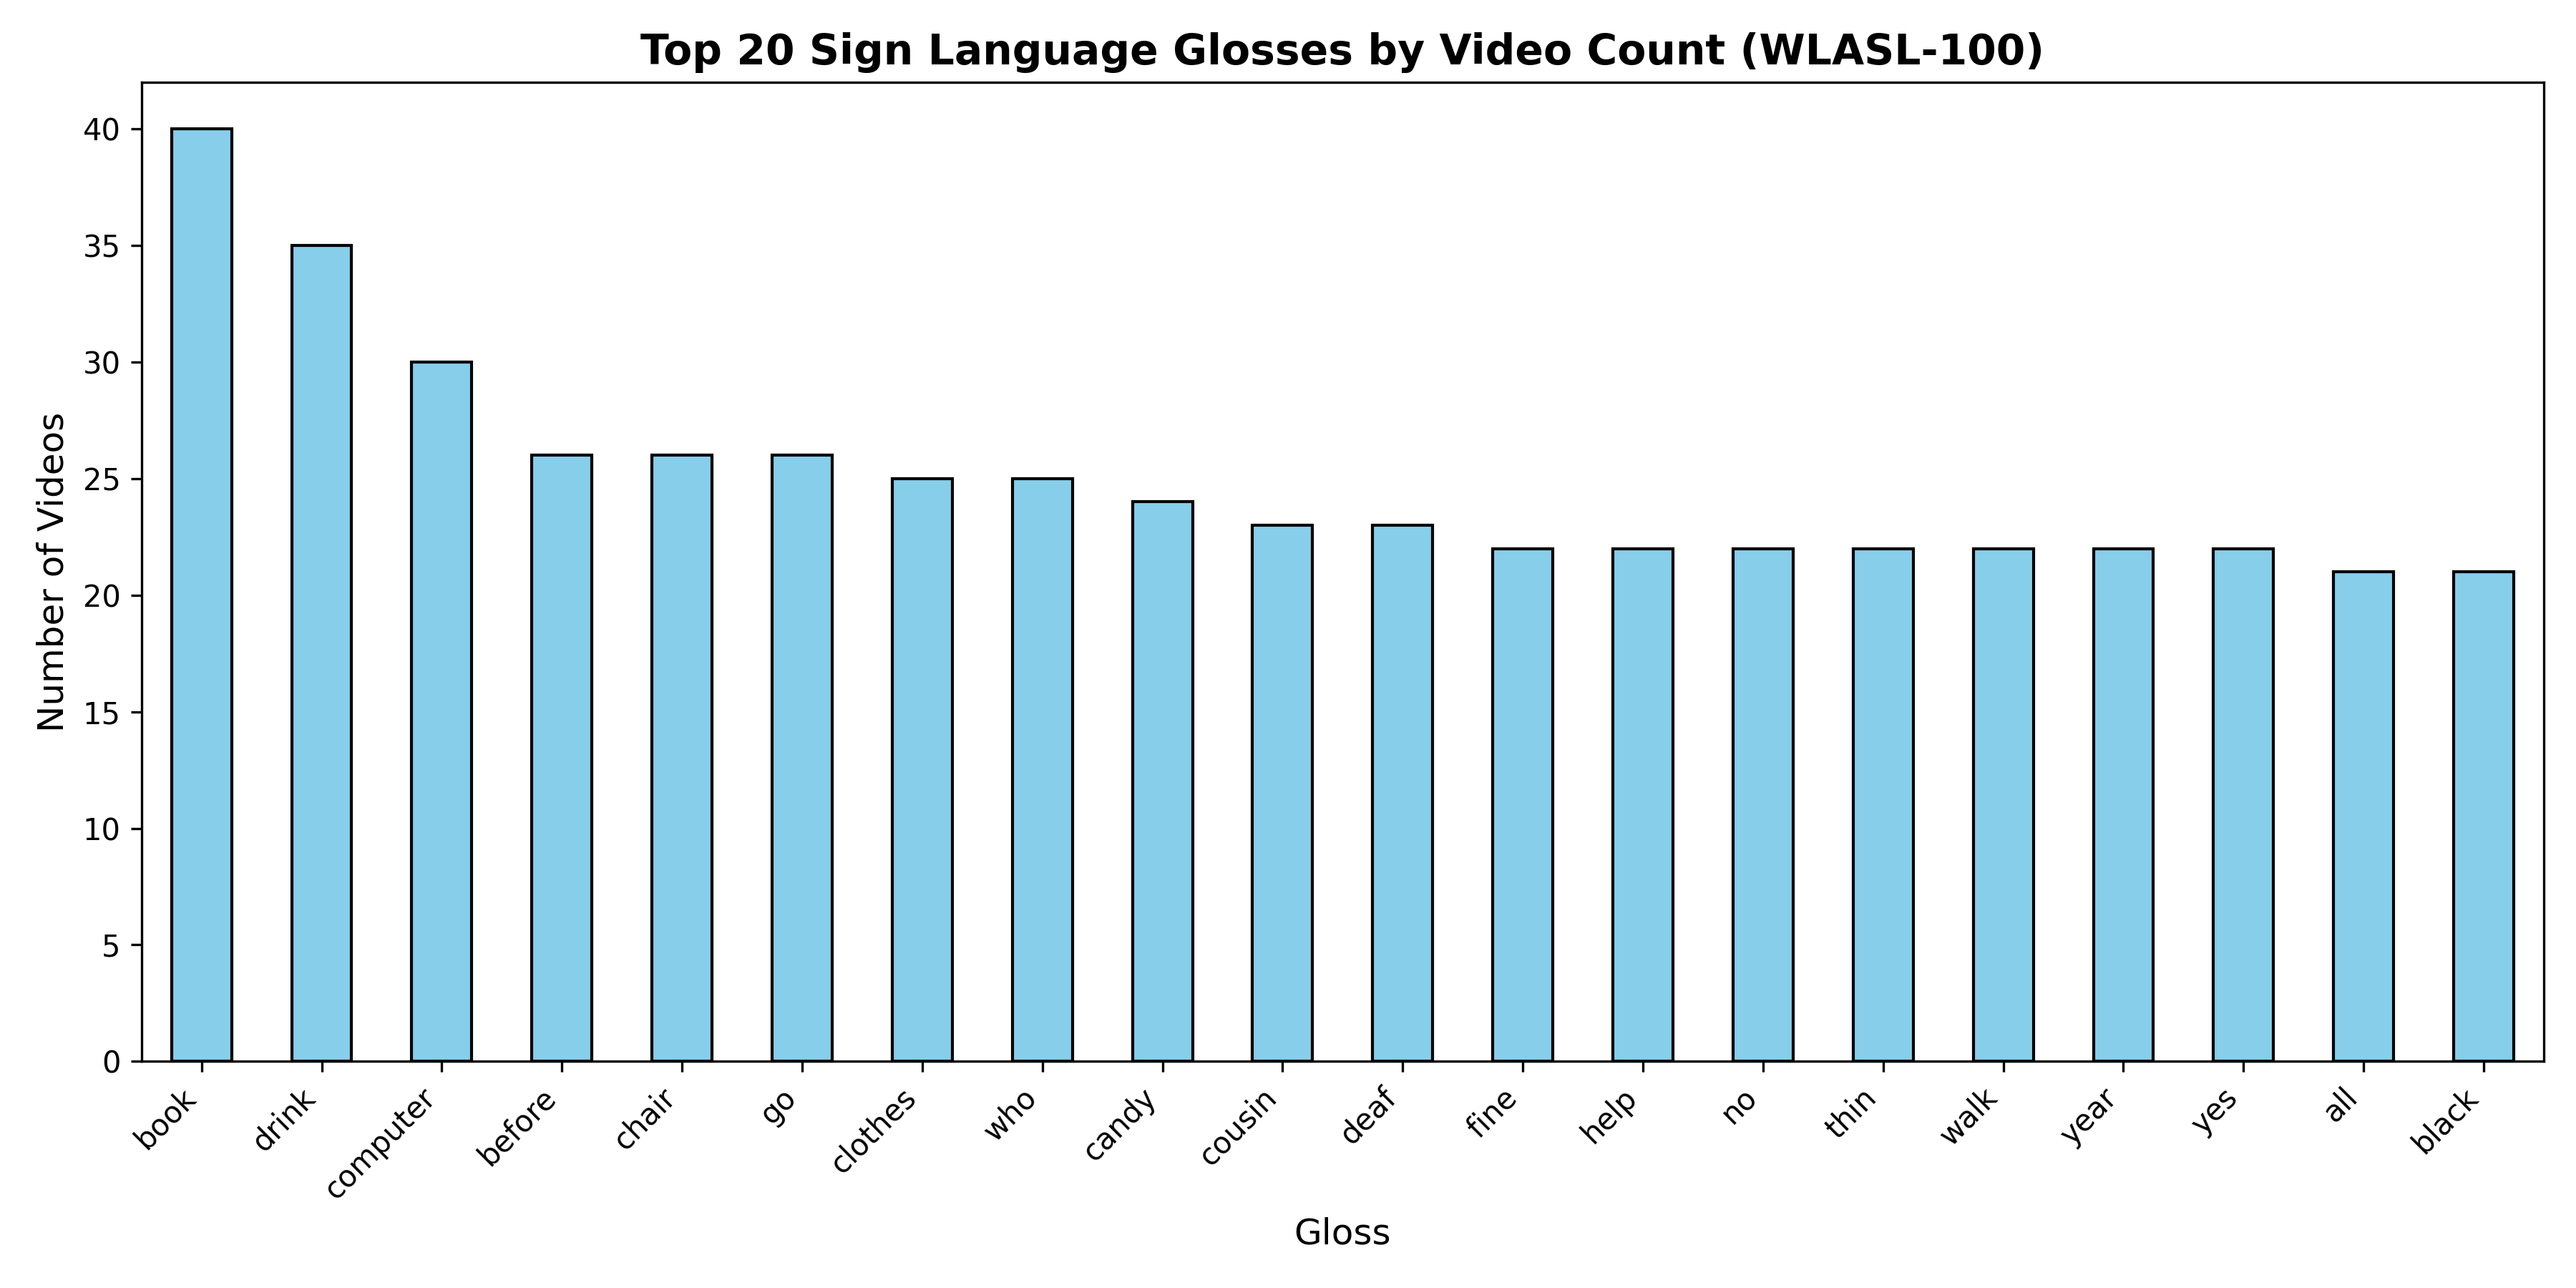
\includegraphics[height=0.6\textheight]{images/top20_glosses.png}
        \caption{Chỉ số F1-Score của Top 20 Glosses}
    \end{figure}
    \textit{Những từ vựng quen thuộc (vd: hello, book) đạt mức nhận diện gần như hoàn hảo (F1 $>$ 0.9).}
\end{frame}

% ==========================================
\section{7. Kết luận và Hướng Phát triển}
% ==========================================
\begin{frame}{Nội dung trình bày}
    \tableofcontents[currentsection, hideallsubsections]
\end{frame}

\begin{frame}{Kết luận Đồ án}
    \begin{enumerate}
        \item Đã xây dựng thành công \textbf{Hệ thống Nhận diện Ngôn ngữ Ký hiệu} hoàn chỉnh, giải quyết bài toán phức tạp từ video RGB $\to$ Khung xương 3D $\to$ Suy luận từ vựng.
        \item Kỹ thuật \textbf{Tiền xử lý Không gian (Spatial Normalization)} đảm bảo tính ổn định bất chấp góc máy và vị trí người quay.
        \item Chứng minh được sự \textbf{áp đảo hoàn toàn của mạng ST-GCN} so với LSTM truyền thống. Việc sử dụng Đồ thị giúp mô hình nắm bắt bản chất vật lý của chuyển động.
        \item Đạt kết quả xuất sắc: \textbf{Top-5 Accuracy $91.5\%$}, đủ điều kiện để ứng dụng vào thực tế làm bộ Gợi ý từ (Autocomplete).
    \end{enumerate}
\end{frame}

\begin{frame}{Định hướng Nghiên cứu Tương lai}
    \begin{itemize}
        \item \textbf{Tích hợp Đặc trưng Khuôn mặt:} Bổ sung 468 điểm Face Mesh từ MediaPipe để học các biểu cảm (ví dụ: nhướn mày, mím môi) - vốn là ngữ điệu của ngôn ngữ ký hiệu.
        \item \textbf{Nhận dạng Câu liên tục (CSLR):} Nâng cấp từ Word-Level lên Continuous Sign Language Recognition, dịch cả một câu dài thay vì chỉ một từ đơn.
        \item \textbf{Triển khai thiết bị Edge (Mobile/IoT):} Thực hiện Lượng tử hóa mô hình (Quantization FP16/INT8) xuất ra ONNX hoặc TensorRT. Khả năng chạy Real-time trên Camera điện thoại mà không cần máy chủ GPU.
    \end{itemize}
\end{frame}

\begin{frame}
    \centering
    \vspace{1cm}
    \LARGE \textbf{Cảm ơn Quý Thầy và các bạn đã lắng nghe!}
    \vspace{1.5cm}
    
    \large \textit{Questions \& Answers}
\end{frame}

\end{document}
